
\documentclass[12pt]{article}
\usepackage{amsmath, amssymb, geometry, fancyhdr}
\usepackage{MnSymbol,wasysym}
\geometry{a4paper, margin=1in}
\setlength{\headheight}{15pt}
\pagestyle{fancy}
\fancyhf{}
\fancyhead[L]{CSCI-769 Quantum Computing Principles and Applications}
\fancyhead[R]{}
\fancyfoot[C]{\thepage}
\newcommand{\bra}[1]{\langle #1 |}
\newcommand{\ket}[1]{| #1 \rangle}
\usepackage{xcolor}
\usepackage{hyperref}
\usepackage{piton}
\usepackage{quantikz}
\usepackage{listings}

\lstset{
    language=Python,
    basicstyle=\ttfamily\small,
    keywordstyle=\color{blue},
    commentstyle=\color{green},
    stringstyle=\color{red},
    numbers=left,
    numberstyle=\tiny\color{gray},
    frame=single,
    breaklines=true,
    captionpos=b
}

\begin{document}

\title{CSCI-769 Quantum Computing Principles and Applications Homework 4}
\author{}
\date{}
\maketitle

\subsection*{1) The Deutsch-Jozsa (DJ) Algorithm (50 pts)}
\textbf{Summary}: The DJ algorithm is interesting because it is an example of how quantum computers can excel at doing certain computational tasks compared to classical computers. If we assume a function $f(x)$ who input space is $2^n$ for some $n$ value. We say the function is constant if for all inputs $f(x)$ returns 0 or 1, respectively. If exactly half the inputs are 0 and the other half are 1, we say the function is balanced. In practice one would need to query $f$ for $2^{n-1}+1$ inputs (half the total inputs plus one) in order to know for certain that $f$ is balanced or constant. Clearly this space is growing exponentially in $n$. With DJ however, one only needs to run the DJ circuit one (and thus queering $f$ once) to achieve the answer on a quantum computer. Neat! This problem will have you explore the circuit, its implementation, and how to convert an "all seeing oracle" to a specific circuit implementation for different instances of $f$. 
\begin{itemize}
    \item a) For each of the f(x), prove $f$ is either constant or balanced where $x_0,x_1 \in \{0,1\}$:
    \begin{itemize}
        \item $f(x_0) = 0$ 
        \item $f(x_0,x_1) = x_0 \oplus x_1 $
        \item $f(x_0) = x_0$ 
        \item $f(x_0,x_1) =1 $
    \end{itemize}.
    \item (b) For every occurrence of $f(x)$, apply the DJ algorithm (as per the circuit outlined below) and ensure the inclusion of the oracle's implementation. Construct and depict the circuit within your solution. Develop a Qiskit program to execute this circuit on both a simulator and an actual NISQ computer for each specific $f$, conducting 20 shots for each simulation and NISQ execution. How does your outcome align with the anticipation from part a)? Hint: Depending on $f(x)$, the oracle might not make any modifications or it could employ $X$ and $CNOT$ gates. Sketch the circuit manually to determine its purpose and design the oracle accordingly.\smiley{}.

    

\end{itemize}
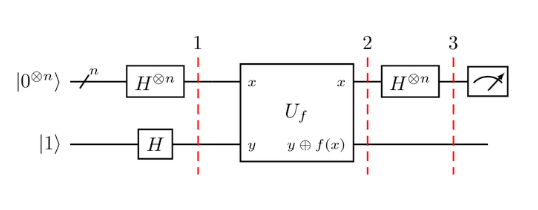
\includegraphics[]{dj.png}

\subsection*{2) Grover's Algorithm (50 pts)}
\textbf{Summary:} Grover's is an example of a quantum algorithm which provides a speedup over a classical algorithm which was thought to be effectively optimal: Making an at least $\mathcal{O}(N)$ complexity cost into $\mathcal{O}(\sqrt{N})$ complexity cost (quadratic time speedup). In this problem we will explore, and appreciate several aspects of the theory of Grover's, and it's practical implementation. 

Consider the Grover Circuit: 

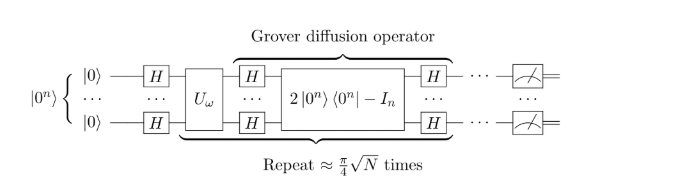
\includegraphics[]{grover.png}

\begin{itemize}
   \item Consider the list $a=[1,2,3,\ldots,2^n]$ where $n=3$. Utilize Qiskit to create Grover's circuit in two scenarios: one to locate the minimum, and another to find the maximum in the list. Remember, you can build these from scratch (figure out how to implement the oracle+diffusion) or leverage Qiskit tools. Assume the Oracle highlights the elements $\ket{000}$ and $\ket{111}$ in each respective case. Tip: Strategically apply some $X$ gates, utilize a $CCZ$ gate, then reverse these with additional $X$ gates. Note: On a real quantum machine, the Oracle magically determines this, but for exploration, we'll know which indices are special to draw some insightful conclusions.
    \item For each circuit, conduct three separate trials whereby the Grover Oracle and Diffusion operation combination is used consecutively for 2, 3, and 8 iterations on the Qiskit simulator with 100 shots (running on the simulator not NISQ device for this experiment). Examine the frequency of Oracle and Diffusion operations to ascertain the measured state. Evaluate how the probability of measuring the marked state varies with the repetition count of Oracle and Diffusion operations. Discuss what occurs when these operations are repeated beyond approximately $\frac{\pi}{4} \sqrt{2^n}$ times—do you enhance the measurement accuracy of the correct state, or does it begin to negatively impact the identification of that state?
    \item While we are conserving our 10-minute allocation for Shor's algorithm, thus not utilizing a NISQ-era device, reflect upon your expectations should these experiments be performed on an authentic NISQ-era quantum computer. Remember from the previous assignment that repeatedly applying gates can lead to cumulative errors. Ideally, in theoretical contexts, Oracle plus Diffusion runs are desired approximately $\sqrt{2^n}$ times, but this comes with potential risks. Consider and comment on this, and why error correction would be required especially when $n$ is large.
\end{itemize}






\subsection*{Understanding $U_{\text{circuit}}^{\dagger}$ of a circuit\texttrademark (50 pts)}
Summary: We are going to appreciate why \textbf{reversible} computing is so important. Its due to the fact you can "undo" things that have been done. Recall from an earlier homework a unitary operation $U$, $UU^\dagger = U^{\dagger}U = I$, which implies $U^{-1}=U^{\dagger}$.

a) Consider the QPE circuit: 

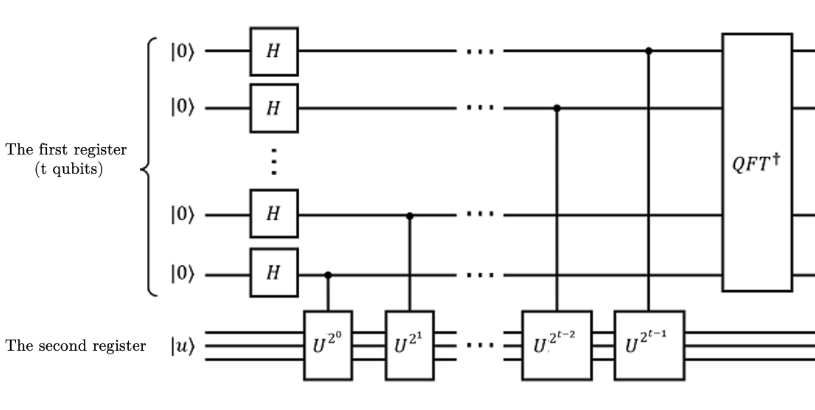
\includegraphics[scale=.35]{QPE.png}

a)Due to the fact a product of unitary operations is unitary, one can imagine the entire application to the circuit to an input as a unitary operation itself. Devise a circuit that undo's the application of $U_{circuit}$ (in this case quantum phase estimation), and display it with Qiskit. For no reason at all lets call this circuit $U_{\text{circuit}}^{\dagger} \smiley{}$. 

b)Show on paper that $U_{\text{circuit}}^{\dagger} U_{\text{circuit}} \ket{0} \ket{u} =\ket{0} \ket{u}  $ by applying the operations of each circuit.

\end{document}


\end{document}
